\documentclass[12pt,a4paper]{article}
\usepackage{cmap}
\usepackage[utf8]{inputenc}
\usepackage[T1,T2A]{fontenc}
\usepackage[english,russian]{babel}
\usepackage{array,booktabs,tabularx}
\usepackage{caption,float,graphicx}
\usepackage{geometry,hyperref,indentfirst,tocloft}
\geometry{margin=25mm}
\hypersetup{unicode=true,colorlinks=true,urlcolor=blue,linkcolor=black}
\setlength{\parindent}{1.25cm}
\setlength{\parskip}{0pt}
\setlength{\emergencystretch}{1em}
\setcounter{tocdepth}{2}
\setlength{\cftbeforesecskip}{5pt}
\setlength{\cftbeforesubsecskip}{1pt}
\renewcommand{\cftsecfont}{\normalsize\bfseries}
\renewcommand{\cftsecpagefont}{\normalsize\normalfont}
\renewcommand{\cftsubsecfont}{\normalsize\normalfont}
\renewcommand{\cftsubsecpagefont}{\normalsize\normalfont}
\renewcommand{\cftdotsep}{1}
\renewcommand{\labelitemi}{\textendash}
\DeclareCaptionLabelSeparator{emdash}{\space---\space}
\captionsetup[figure]{justification=centering,singlelinecheck=false,labelsep=emdash}
\addto\captionsrussian{\renewcommand{\figurename}{Рис.}}
\newcommand{\code}[1]{\texttt{\detokenize{#1}}}
\newcolumntype{P}[1]{>{\raggedright\arraybackslash}p{#1}}
\newcommand{\ReportDate}{21.10.2026}
\newcommand{\ExperimentDate}{21 октября 2026 года}
\newcommand{\CorpusDocumentCount}{12497}
\newcommand{\CorpusDocuments}{12\,497}
\newcommand{\CorpusTitleOnly}{121}
\newcommand{\CorpusKB}{40\,324,69}
\newcommand{\TokenCount}{4\,140\,679}
\newcommand{\MeanTokenLength}{5,308}
\newcommand{\ProcessingMs}{389,638}
\newcommand{\ElapsedMs}{431,545}
\newcommand{\ThroughputKB}{93\,442,7}
\newcommand{\MsPerKB}{0,0107}
\newcommand{\OutputElapsedMs}{1\,581,327}
\newcommand{\ProcessWallMs}{441,188}
\newcommand{\OutputWallMs}{1\,594,473}
\newcommand{\BenchmarkRuns}{5}

\newcommand{\LabSourceRows}{%
Eurogamer & 1058 & 521\,285 & 4,682 \\
GameMAG & 2442 & 482\,025 & 5,700 \\
GamingOnLinux & 378 & 121\,603 & 4,734 \\
Игромания & 2411 & 731\,247 & 5,734 \\
IXBT.games & 1817 & 338\,056 & 5,880 \\
PC Gamer & 1477 & 888\,458 & 4,625 \\
PlayGround & 1290 & 215\,523 & 5,858 \\
StopGame & 1624 & 842\,482 & 5,537 \\
}

\newcommand{\LabTimingRows}{%
1563 & 5\,147,28 & 51,415 & 57,767 & 89\,104,9 \\
3125 & 9\,682,72 & 100,796 & 114,002 & 84\,934,6 \\
6249 & 19\,961,70 & 199,960 & 224,238 & 89\,020,3 \\
12497 & 40\,324,69 & 389,638 & 431,545 & 93\,442,7 \\
}

\newcommand{\LabTestCount}{30}


\begin{document}
\hypersetup{pageanchor=false}
\begin{titlepage}
\begin{center}
{\large МОСКОВСКИЙ АВИАЦИОННЫЙ ИНСТИТУТ\\
(НАЦИОНАЛЬНЫЙ ИССЛЕДОВАТЕЛЬСКИЙ УНИВЕРСИТЕТ)}

\vspace{18pt}
{\large Факультет информационных технологий и прикладной математики}

{\large Кафедра вычислительной математики и~программирования}

\vfill
{\large\textbf{Лабораторная работа №3 по курсу\\ «Информационный поиск»}}

\vspace{12mm}
{\large\textbf{Токенизация}}

\vfill
\begin{flushright}
\begin{tabular}{@{}r@{:\hspace{0.6em}}l@{}}
\textit{Студент} & К.\,А. Арусланов\\
\textit{Группа} & М8О-403Б-23\\
\textit{Преподаватель} & А.\,А. Кухтичев\\
\textit{Дата} & \ReportDate\\
\textit{Оценка} &
\end{tabular}
\end{flushright}
\vfill
Москва, 2026
\end{center}
\end{titlepage}
\hypersetup{pageanchor=true}
\setcounter{page}{2}
\tableofcontents
\newpage

\section{Постановка задачи}

Нужно реализовать процесс разбиения текстов документов на токены, который
потом будет использоваться при индексации. Для этого потребуется выработать
правила, по которым текст делится на токены. Необходимо описать их в отчёте,
указать достоинства и недостатки выбранного метода. Привести примеры токенов,
которые были выделены неудачно, объяснить, как можно было бы поправить
правила, чтобы исправить найденные проблемы.

В результатах выполнения работы нужно указать следующие статистические данные:
\begin{itemize}
\item количество токенов;
\item среднюю длину токена.
\end{itemize}

Кроме того, нужно привести время выполнения программы, указать зависимость
времени от объёма входных данных. Указать скорость токенизации в расчёте на
килобайт входного текста. Является ли эта скорость оптимальной? Как её можно
ускорить?

\section{Метод решения}

\subsection{Корпус и подготовка данных}

Темой корпуса являются русскоязычные и англоязычные публикации о компьютерных
играх восьми источников. Входные данные --- публикации, сохранённые роботом
второй работы в коллекции \code{documents} базы MongoDB. Используются только
пригодные для индексации записи без ошибки парсера. Из каждой записи
экспортируются заголовок и основной текст. Публикации без основного текста
участвуют заголовком; страницы-каталоги исключаются до токенизации.

Python-экспортёр создаёт неизменяемый локальный снимок с бинарным файлом
\code{corpus.bin}, таблицей соответствия ID и URL \code{documents.jsonl}
и описанием \code{manifest.json}. Для снимка сохраняется SHA-256.
В бинарном формате поля предваряются длинами в байтах, поэтому переводы
строк и нулевые символы не нарушают границы документов. Заголовок и основной
текст остаются отдельными полями. Сырой HTML при этом не читается.

Экспорт идёт курсором MongoDB, обработка --- по одному документу.
Весь корпус не требуется помещать в оперативную память. Снимок позволяет
повторять измерения на одинаковых данных и исключить MongoDB из замеров
производительности токенизатора. Экспорт не меняет базу. В описании снимка
зафиксированы начало и конец экспорта. Обычный курсор не создаёт
транзакционный снимок MongoDB: при одновременной обкачке состав базы может
меняться. Все приведённые подсчёты относятся к завершённому локальному файлу.

\subsection{Алгоритм и правила}

Основная программа написана на C++17 с использованием разрешённой для
токенизации STL. Алгоритм самостоятельно декодирует UTF-8 и последовательно
просматривает кодовые точки. Версия правил обозначена \code{gaming-v3}.

\begin{itemize}
\item Буквы ASCII, русские буквы, латиница Latin-1 и Extended-A, а также
ASCII-цифры входят в состав слов. Цифры сохраняются и внутри названий:
\code{PS5} превращается в \code{ps5}, \code{3D} --- в \code{3d}.
\item Регистр нормализуется по явным таблицам поддерживаемых букв, независимо
от локали системы. Буква «ё» не заменяется на «е».
\item Внутренние дефисы и апострофы сохраняются. Типографские апострофы
приводятся к ASCII-апострофу, обычный и неразрывный дефисы --- к \code{-}.
Соединитель допустим только внутри слова перед буквой или цифрой.
Среднее и длинное тире считаются разделителями.
\item Обозначения \code{C++}, C\# и их варианты с номером стандарта,
например \code{C++17}, сохраняются целиком. Правило применяется к отдельному
\code{C}/\code{c}, а не к любой последовательности букв перед плюсом.
\item В числовой последовательности точка сохраняется перед следующей цифрой:
\code{3.0.1} становится одним токеном. Поддерживается префикс \code{v},
например \code{V1.2.3} превращается в \code{v1.2.3}. Конечная точка
предложения отделяется. Это лексическое правило: десятичные числа и IP-адреса
также сохраняются целиком, без определения типа сущности.
\item Цепочка из трёх и более одиночных букв через точки превращается
в один токен без точек: \code{S.T.A.L.K.E.R.} и \code{STALKER} дают
одинаковый терм \code{stalker}. Конечная точка необязательна.
Две буквы через точку не склеиваются, многобуквенные сегменты не
распознаются как такая цепочка. Правило действует на поддерживаемую
латиницу и русские буквы, без словаря названий игр.
\item Пробелы, переводы строк, остальная пунктуация и emoji разделяют слова.
Стоп-слова, короткие слова и числа не удаляются.
\item Комбинируемые знаки U+0300--U+036F присоединяются к начатому токену.
Unicode-нормализация NFC/NFKC не выполняется. Остальные письменности пока
считаются разделителями; полное Unicode case folding не реализовано.
\item Повреждённый UTF-8 и обрезанный бинарный формат считаются ошибкой
входных данных. Программа завершается с ненулевым кодом возврата.
\end{itemize}

Каждый токен содержит ID документа, имя поля, позицию с нуля внутри поля,
начальное и конечное байтовые смещения и нормализованный терм. Смещения
относятся к исходному тексту, а не к строке после нормализации.
Такое представление можно использовать при построении позиционного индекса
и сниппетов. Тот же модуль подходит для обработки поисковых запросов.
Лемматизация и стемминг в этой работе не выполняются.

Просмотр занимает линейное время относительно числа байтов текста.
В памяти остаются текущий документ и буфер токена; глобальный словарь
терминов не строится. Длина токена считается в кодовых точках нормализованной
строки, включая внутренние соединители, а не в байтах UTF-8. Это также
не число видимых графем: буква и отдельный комбинируемый знак дают две
кодовые точки. Средняя длина равна отношению суммы длин токенов к их
количеству; при отсутствии токенов принимается равной нулю.

\subsection{План тестирования и измерений}

CLI-тесты проверяют русский и английский текст, регистр и «ё», цифры,
типографские соединители, обозначения языков программирования, версии,
цепочки одиночных букв через точки,
диакритику, границы UTF-8, позиции внутри полей,
пустые и большие тексты. Отдельно проверяются повреждённая кодировка,
обрезанные записи, недопустимые длины, неверные аргументы, сохранение
существующих файлов и отсутствие опубликованного частичного результата
после ошибки. Тесты экспортёра проверяют отбор документов, сохранение
публикаций с одним заголовком и отсутствие изменений в базе. Тесты
демонстрации проверяют соответствие фрагмента исходной статье,
байтовые границы, выбор документа и вывод UTF-8.

Для измерения зависимости времени от размера берутся каждый восьмой,
четвёртый, второй документ снимка и весь снимок. Подвыборки распределены
по исходному порядку URL, поэтому включают разные сайты. Тексты не
дублируются для искусственного увеличения объёма. На каждой подвыборке
проводится один прогрев и \BenchmarkRuns{} измерений; основным результатом
служит медиана. Все повторы сохраняются в \code{benchmark.json}.

Отдельно измеряется сканирование с нормализацией и счётчиками, а также
полное чтение и обработка бинарного файла. В этих повторах запись токенов
выключена. Ещё один запуск сохраняет полный TSV и показывает стоимость
вывода. Создание процесса и экспорт MongoDB в приведённое внутреннее
время не входят. Файловый кеш прогрет; результаты не характеризуют чтение
с холодного диска. Везде используется десятичный килобайт: 1 КБ = 1000 байт.

\section{Результаты}

\subsection{Количество и длина токенов}

Эксперимент выполнен \ExperimentDate{} на снимке из \CorpusDocuments{}
публикаций, из них \CorpusTitleOnly{} содержат только заголовок. Суммарный
размер заголовков и основного текста --- \CorpusKB{} КБ. Статистика
рассчитывается по обоим полям без удаления стоп-слов и словоформ.

\begin{center}
\begin{tabular}{lr}
\toprule
Показатель & Значение \\
\midrule
Количество документов & \CorpusDocuments \\
Количество токенов & \TokenCount \\
Средняя длина токена, кодовых точек & \MeanTokenLength \\
\bottomrule
\end{tabular}
\end{center}

\begin{center}
\small
\begin{tabular}{lrrr}
\toprule
Источник & Документы & Токены & Средняя длина \\
\midrule
\LabSourceRows
\bottomrule
\end{tabular}
\end{center}

Статистика получена по всем пригодным записям завершённого экспорта.
\ifnum\CorpusDocumentCount<30000
Объём пока не достигает требуемых курсом 30--50 тысяч документов.
После продолжения обкачки необходимо повторить экспорт и тот же эксперимент.
\else
Корпус достиг минимального объёма в 30 тысяч реальных документов.
\fi
Копии текстов для увеличения числа документов не добавлялись.

\subsection{Производительность}

Программа собрана с оптимизацией \code{-O3} и стандартом C++17 на Windows
AMD64. Точная версия компилятора, его флаги и SHA-256 бинарного файла
сохранены вместе с результатами. Объём в таблице включает только UTF-8
заголовки и тексты, без служебных полей бинарного формата.

\begin{center}
\small
\setlength{\tabcolsep}{5pt}
\begin{tabular}{rrrrr}
\toprule
Документы & Текст, КБ & Обработка, мс & С чтением, мс & Скорость, КБ/с \\
\midrule
\LabTimingRows
\bottomrule
\end{tabular}
\end{center}

На всём снимке медиана времени обработки составляет \ProcessingMs{} мс,
с чтением --- \ElapsedMs{} мс. Скорость чтения и обработки равна
\ThroughputKB{} КБ/с, или \MsPerKB{} мс/КБ. Запуск с сохранением полного
TSV занимает \OutputElapsedMs{} мс: форматирование и запись результата
добавляют работу, которой нет в измерениях без вывода.
По внешнему таймеру медиана полного запуска без TSV составляет
\ProcessWallMs{} мс, а отдельный запуск с TSV --- \OutputWallMs{} мс.
Эти значения дополнительно включают создание процесса и передачу его
небольшого JSON-ответа вызывающему Python-скрипту.

\begin{figure}[H]
\centering
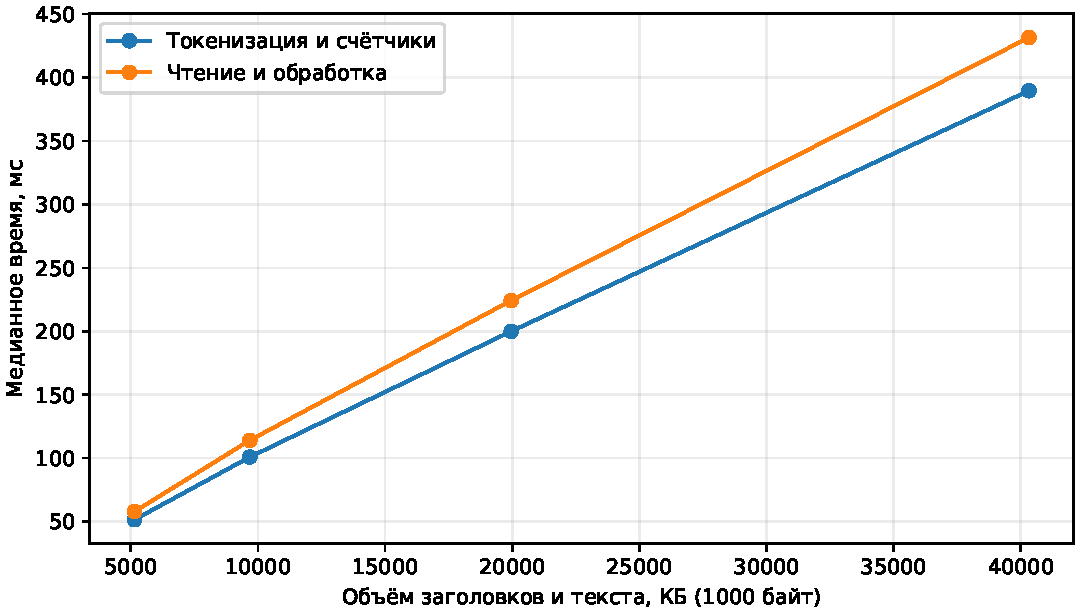
\includegraphics[width=0.95\linewidth]{lab3/timing.pdf}
\caption{Зависимость медианного времени от объёма входного текста.}
\end{figure}

Линейный проход соответствует ожидаемой зависимости порядка $O(B)$,
где $B$ --- объём текста. На небольших подвыборках также влияют накладные
расходы, состав русских и английских текстов и планирование процессов.
Четырёх измеряемых объёмов недостаточно для вывода о скорости
на миллионном корпусе.

По порядку сложности полный просмотр текста улучшить нельзя: нужно
прочитать входные символы. При этом измеренная реализация не доказана
оптимальной по постоянным затратам. Возможные ускорения --- отдельный
быстрый путь для ASCII, уменьшение расходов вызова обработчика токенов
и пакетная запись более компактного результата. Параллельная обработка
независимых документов также возможна; сравнивать её следует отдельным
экспериментом с теми же правилами и проверкой одинакового результата.

\subsection{Качество выделения и ограничения}

В сохранённых публикациях найдены следующие характерные случаи.
Короткие фрагменты и ожидаемый результат включены в CLI-тесты.

\begin{center}
\small
\renewcommand{\arraystretch}{1.16}
\begin{tabularx}{\textwidth}{@{}P{0.19\textwidth}P{0.22\textwidth}X@{}}
\toprule
Фрагмент & Результат & Наблюдение и возможное улучшение \\
\midrule
\code{C++}, C\# (PC Gamer) & \code{c++}, \texttt{c\#} & В первой версии оба
обозначения превращались в \code{c}. Добавлено правило сохранения
специальных суффиксов; теперь три названия различаются. \\
\code{3.0.1} (GameMAG) & \code{3.0.1} & В первой версии получались три
числа. Теперь точка между цифрами сохраняется, а конечная точка
предложения отделяется. \\
\code{S.T.A.L.K.E.R.} & \code{stalker} &
Цепочка одиночных букв теперь распознаётся целиком. Точки удаляются,
поэтому написание \code{STALKER} даёт тот же терм. \\
\code{Half-Life} (GameMAG) & \code{half-life} & Название сохраняется,
но запрос \code{Half Life} даёт два токена. Для сопоставления вариантов
понадобится согласованное правило альтернативного представления. \\
\texttt{\fontencoding{T1}\selectfont Pok\'emon} (IXBT.games) &
\texttt{\fontencoding{T1}\selectfont pok\'emon} & Диакритика сохраняется;
\code{Pokemon} будет другим термом. Возможен отдельный вариант без диакритики,
но его следует оценить на неоднозначных названиях. \\
\bottomrule
\end{tabularx}
\end{center}

Пример с C++ и C\# взят из
\href{https://www.pcgamer.com/if-it-werent-for-ram-there-would-be-70-fewer-windows-patches/}{публикации PC Gamer},
версия --- из
\href{https://gamemag.ru/news/163686/playstation-5-destruction-all-stars-free-2-play}{новости GameMAG о Destruction AllStars}.
Положительные примеры ---
\href{https://gamemag.ru/news/116043/black-mesa-novyy-skrinshot-glavy-xen}{новость GameMAG о Black Mesa}
и \href{https://ixbt.games/news/2026/04/01/408172-patentnoe-vedomstvo-ssa-otozvalo-patent-nintendo-na-igrovuiu-mexaniku-prizyva-personazei.html}{материал IXBT.games о патенте Nintendo}.

Название \code{S.T.A.L.K.E.R.} встречается и в сохранённой
\href{https://gamemag.ru/news/11344/pobediteli-kri-awards-2004}{публикации GameMAG о КРИ Awards}.
Его нормализация демонстрируется на исходном фрагменте этой статьи.
Обратная сторона общего правила --- \code{a.b.c} также даст \code{abc},
даже если это инициалы или части доменного имени. Для различения
таких случаев понадобились бы дополнительные ограничения или контекст.
Другие ограничения --- неполный
набор письменностей и отсутствие NFC. Новые правила нужно применять
одинаково к документам и запросам, меняя версию токенизатора.

\subsection{Автотесты и воспроизведение}

Успешно выполнены \LabTestCount{} автоматических тестов экспортёра,
CLI токенизатора и демонстрации.
Часть тестов содержит несколько входных случаев. Полный журнал приложен
как \code{doc/lab3/tests.txt}; данные эксперимента находятся в
\code{statistics.json}, \code{benchmark.json} и \code{benchmark.csv}
того же каталога. Сборка, тесты, экспорт и замеры запускаются одной командой:

\begin{verbatim}
python run_lab3.py --config crawler.large.yaml \
  --output data/tokenization/run_001 --report-dir doc/lab3
\end{verbatim}

В примере перенос строки дан для оболочки Bash; команду также можно
ввести одной строкой. Требования и отдельные команды описаны в
\code{doc/lab3_run.md}. Снимки корпуса и полные токены хранятся локально
в \code{data/tokenization/} и не включаются в Git.

Для демонстрацииs достаточно команды:
\begin{verbatim}
python demo_lab3.py
\end{verbatim}
Она выбирает реальные статьи из последнего локального снимка и выводит
источник, ID, заголовок, URL, исходный фрагмент и таблицу токенов.
Колонка \code{original} извлекается из исходного текста по байтовым
границам, возвращённым C++-программой. Позиции и смещения относятся
к целому полю статьи, а не к началу показанного фрагмента.
Демонстрируются версии, обозначения языков и нормализация названий
с точками. Произвольный документ
можно выбрать опцией \code{--document-id}, фрагмент --- опцией \code{--find}.

Исходный код и отчёт предназначены для ветки \code{lab3}:
\url{https://github.com/kirbasss/MAI-IR/tree/lab3}.

\begin{figure}[H]
\centering
\href{https://github.com/kirbasss/MAI-IR/tree/lab3}{
\includegraphics[width=28mm]{img/qr_lab3.png}}
\caption{QR-код для перехода к ветке \code{lab3} репозитория.}
\end{figure}

\section{Вывод}

В этой работе я реализовал токенизацию игровых публикаций и проверил её
на русских и английских текстах. Было интересно увидеть, что даже простое
разбиение на слова требует нескольких решений: сохранять ли дефис,
как обрабатывать апострофы и что делать с цифрами в названиях игр.
Особенно наглядными оказались C++ и C\#: сначала после удаления пунктуации
они превращались в одинаковый токен. Я уточнил правила, и теперь эти
обозначения, как и номера версий игр, сохраняются целиком. Для названий
вроде \code{S.T.A.L.K.E.R.} я добавил объединение одиночных букв через
точки: теперь их можно сопоставлять с обычным написанием без точек.

Я получил статистику токенов, измерил скорость обработки и подготовил
повторяемый запуск экспериментов и демонстрацию на настоящих статьях.
Позиции и исходные границы слов сохранены,
поэтому результат можно использовать в следующих работах. Дальше нужно
расширить реально скачанный корпус, повторить измерения и отдельно
добавить обработку словоформ, сохранив возможность точного сопоставления.

\end{document}
